% Copyright (c) 2026 CorrectBrain
% SPDX-License-Identifier: MIT

\PassOptionsToPackage{dvipsnames,svgnames,x11names}{xcolor}
\documentclass[tikz,border=8pt]{standalone}
\usetikzlibrary{arrows.meta,positioning,calc,shapes,shadows,decorations.pathmorphing,shapes.geometric,backgrounds,decorations.markings,decorations.pathreplacing,decorations.text,fit,shapes.misc,shapes.arrows,matrix,bending,3d,chains,intersections,shapes.symbols,svg.path,shapes.multipart,snakes,shapes.callouts,angles,quotes}
\usetikzlibrary{fadings,shadows.blur,patterns,patterns.meta}

\usepackage{amsmath}
\usepackage{amssymb}
\usepackage{fontawesome5}
\usepackage{xcolor}

\providecolor{gold}{RGB}{212,175,55}
\providecolor{silver}{RGB}{192,192,192}
\providecolor{bronze}{RGB}{205,127,50}
\providecolor{darkblue}{RGB}{0,0,139}
\providecolor{lightblue}{RGB}{173,216,230}
\providecolor{darkgreen}{RGB}{0,100,0}
\providecolor{lightgreen}{RGB}{144,238,144}
\providecolor{darkred}{RGB}{139,0,0}
\providecolor{navy}{RGB}{0,0,128}
\providecolor{skyblue}{RGB}{135,206,235}
\providecolor{beige}{RGB}{245,245,220}
\providecolor{cream}{RGB}{255,253,208}

% --- DEFINE CUSTOM COLOR PALETTE ---
\definecolor{gridgray}{RGB}{224, 224, 224}
\definecolor{mathred}{RGB}{211, 47, 47}
\definecolor{mathblue}{RGB}{25, 118, 210}
\definecolor{mathgreen}{RGB}{56, 142, 60}
\definecolor{textdark}{RGB}{50, 50, 50}

\begin{document}
\begin{tikzpicture}[
    xscale=1, yscale=-1,
    font=\sffamily,
    % --- STYLES ---
    point/.style={circle, fill=black, inner sep=2pt},
    bubble/.style={
        draw=black!15, fill=white, rounded corners=8pt,
        inner sep=10pt, font=\sffamily\small,
        blur shadow={shadow opacity=12, shadow yshift=-4pt, shadow xshift=0pt, shadow blur radius=3pt}
    }
]

% --- BACKGROUND CANVAS (STRICT WHITE) ---
\fill[white] (-5, -6) rectangle (22, 12);

% --- TITLES & TYPOGRAPHY ---
\node[font=\Huge\bfseries\sffamily\color{textdark}, anchor=center] at (9.5, -4.5) {The Geometric Vector of \texttt{height: auto}};
\node[font=\large\sffamily\color{gray}, anchor=center] at (9.5, -3.5) {Tracking the bottom-right coordinate $C(x,y)$ of the bounding box during fluid scale};

% --- GRID & AXES (DOM FLOW) ---
% Grid Matrix
\foreach \x in {1,2,...,11} {
    \draw[color=gridgray, line width=0.5pt, opacity=0.5] (\x, 0) -- (\x, 9);
}
\foreach \y in {1,2,...,9} {
    \draw[color=gridgray, line width=0.5pt, opacity=0.5] (0, \y) -- (11, \y);
}

% X-Axis and Y-Axis (DOM Flow Downward)
\draw[-Stealth, very thick, textdark] (0, -0.1) -- (11.5, -0.1);
\node[anchor=south east, font=\sffamily\bfseries\color{textdark}] at (11.5, -0.4) {X-Axis (Width)};

\draw[-Stealth, very thick, textdark] (-0.1, 0) -- (-0.1, 9.5);
\node[anchor=north east, font=\sffamily\bfseries\color{textdark}] at (-0.3, 9.5) {Y-Axis (Height) - DOM Flow};

% --- DIMENSION BRACES ---
% Wr (Blue Top Brace)
\draw[mathblue, thick, decorate, decoration={brace, amplitude=4pt}] (0, -1.0) -- (4, -1.0);
\node[font=\sffamily\bfseries\color{mathblue}, anchor=south] at (2, -1.4) {$W_r$};

% Wi (Red Top Brace)
\draw[mathred, thick, decorate, decoration={brace, amplitude=5pt}] (0, -2.2) -- (8, -2.2);
\node[font=\sffamily\bfseries\color{mathred}, anchor=south] at (4, -2.6) {$W_i$};

% Hr (Blue Left Brace)
\draw[mathblue, thick, decorate, decoration={brace, amplitude=4pt}] (-1.0, 3) -- (-1.0, 0);
\node[font=\sffamily\bfseries\color{mathblue}, anchor=east] at (-1.4, 1.5) {$H_r$};

% Hi (Red Left Brace)
\draw[mathred, thick, decorate, decoration={brace, amplitude=5pt}] (-2.2, 6) -- (-2.2, 0);
\node[font=\sffamily\bfseries\color{mathred}, anchor=east] at (-2.6, 3) {$H_i$};

% --- GEOMETRY BOXES ---
% Intrinsic Box (Red)
\draw[draw=mathred, very thick, fill=mathred, fill opacity=0.05, rounded corners=2pt] (0, 0) rectangle (8, 6);

% Stylized Source Image Placeholder Icon inside Intrinsic Box
\begin{scope}[shift={(2, 4.5)}, yscale=-1, scale=0.6, opacity=0.15, textdark, line width=1.5pt]
    \fill[textdark] (-1.8, -1.2) -- (-0.4, 0.6) -- (0.5, -0.4) -- (1.2, 0.4) -- (2.0, -1.2) -- cycle;
    \fill[textdark] (1.3, 1.1) circle (0.35);
\end{scope}

\node[font=\sffamily\bfseries\color{mathred!80!black}, anchor=center] at (3, 5.5) {Intrinsic Bounding Box};

% Intrinsic Corner Point Ci
\node[point, fill=mathred, minimum size=6pt] at (8, 6) {};
\node[anchor=south west, font=\sffamily\bfseries\color{mathred}] at (8.2, 5.8) {$C_i (W_i, H_i)$};

% Rendered Box (Blue)
\draw[draw=mathblue, very thick, fill=mathblue, fill opacity=0.15, rounded corners=2pt] (0, 0) rectangle (4, 3);
\node[font=\sffamily\bfseries\color{mathblue!90!black}, anchor=center] at (2, 1.5) {Rendered Box};

% Rendered Corner Point Cr
\node[point, fill=mathblue, minimum size=6pt] at (4, 3) {};
\node[anchor=south east, font=\sffamily\bfseries\color{mathblue}] at (3.8, 2.8) {$C_r (W_r, H_r)$};

% --- THE MATHEMATICAL VECTOR LINE ---
\draw[dashed, mathgreen, line width=2pt, -Stealth] (0, 0) -- (10, 7.5);
\node[anchor=west, align=left, font=\sffamily\bfseries\color{mathgreen}] at (10.5, 7.5) {Constant Aspect Ratio\\Vector Line};

% --- INFORMATION BUBBLES & ARROW ROUTING ---
% Red Bubble (Zero Pixel Distortion) - Relocated to TOP
\node[bubble, text width=7cm, draw=mathred] (lockBubble) at (14.8617,2.4817) {
    \textbf{\color{mathred}\faLock\ Zero Pixel Distortion}\\[3pt]
    Because the coordinate scales perfectly along the vector line, the pixel matrix is never squished or stretched. This is the core engine of flexible media in responsive web design.
};
\draw[-Stealth, thick, mathred] (lockBubble.west) -- (6, 2.5) |- (4.1, 2.9);

% Green Bubble (Linear Trajectory Mapping) - Relocated to BOTTOM
\node[bubble, text width=7cm, draw=mathgreen] (mathBubble) at (18.8152,7.5971) {
    \textbf{\color{mathgreen}\faCodeBranch\ Linear Trajectory Mapping}\\[3pt]
    The bottom-right coordinate $C(x,y)$ must always lie on the straight line defined by the aspect ratio. \\[5pt]
    Equation of the Vector Line:\\[2pt]
    $\mathbf{y = \left( \frac{H_i}{W_i} \right) x}$\\[5pt]
    \texttt{height: auto} acts as a mathematical constraint, forcing $H_r$ to calculate onto this exact line.
};
\draw[-Stealth, thick, mathgreen] (mathBubble.west) -- (9.5, 7.5) |- (7.1, 5.25);

\end{tikzpicture}
\end{document}
